\chapter{Methodology}
\section{Problem Formulation}
\subsection{Feature Matching as Correspondence Prediction}
The current solution implemented at SteelSeries leverages SIFT (Scale-Invariant
Feature Transform) for detecting specific icons and matching them across frames
in a live video feed. This method was selected due to its well-documented
robustness to scale, rotation, and illumination changes, which is critical in
dynamic gaming environments where UI elements may vary slightly between frames
or scenes. Unlike deep learning-based object detectors such as YOLO (You Only
Look Once) or SSD (Single Shot MultiBox Detector), which require large
annotated datasets and frequent re-training to adapt to new games, graphical
updates, or icon variations—SIFT operates in a fully handcrafted and
deterministic manner, making it model-free and highly generalizable. Its
independence from external data or pre-trained models ensures long-term
maintainability and consistency, especially in production systems that must
support a wide range of games without frequent intervention. Moreover, feature
matching methods like SIFT allow us to establish correspondences between
keypoints in a pair of images without prior training, enabling quick deployment
and adaptability. This is particularly advantageous in scenarios where the
visual elements to be detected (such as achievement badges, in-game items, or
menu icons) are not part of a predefined object class and may appear in various
sizes or partially occluded contexts. The matching process, relying purely on
local feature descriptors, operates seamlessly and with minimal setup, reducing
engineering overhead while maintaining high matching accuracy. However, while
SIFT is reliable, its computational cost—especially on CPU-bound systems
without GPU acceleration—poses challenges for real-time performance at high
frame rates, motivating the exploration of neural-assisted or hybrid approaches
that can retain robustness while improving throughput.
\subsection{Objectives in Terms of Speed, Accuracy, and Robustness}

\subsubsection{Performance Requirements}
To establish a comprehensive evaluation framework, we define specific
performance targets that the enhanced system must achieve across three key
dimensions:

\begin{table}[h]
    \centering
    \begin{tabular}{|l|c|c|c|c|c|}
        \hline
        \textbf{Image Size}   & 1280×720 & 960×540 & 640×360 & 320×180 & 128×72  \\
        \hline
        \textbf{Scale}        & 100\%    & 75\%    & 50\%    & 25\%    & 10\%    \\
        \hline
        \textbf{KPs detected} & 636      & 534     & 403     & 155     & 46      \\
        \hline
        \textbf{Time}         & 0.0837s  & 0.0470s & 0.0226s & 0.0082s & 0.0025s \\
        \hline
    \end{tabular}
    \caption{Performance Requirements and Current Baseline Comparison}
    \label{tab:performance_requirements}
\end{table}
\subsection{Choice of Models}
Although each Neural Network solution excel in different aspects, we have to
select a model that balances speed, accuracy, and robustness. The chosen model
should be lightweight enough to run efficiently on CPU while still providing
high matching precision and recall across various game icons and UI elements.
Among the available options, we considered \textbf{XFeat} as our primary
candidate due to its proven performance.
\begin{figure}[h]
    \centering
    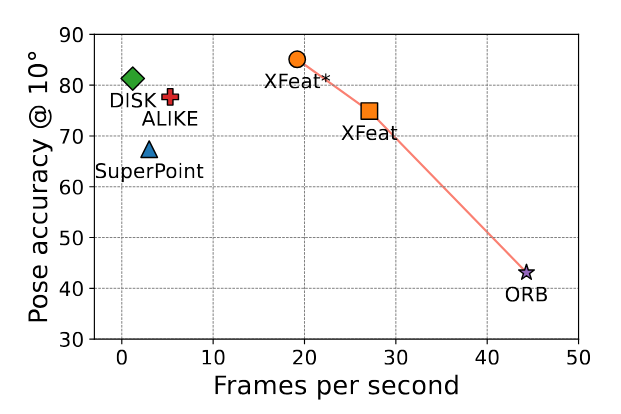
\includegraphics[width=0.8\textwidth]{ressources/xfeat-comparative-graph.png}
    \caption{Comparison of XFeat with other feature matching methods}
    \label{fig:xfeat_architecture}
\end{figure}
\subsection{Datasets}
XFeat utilizes two primary datasets for training and evaluation: the MegaDepth
dataset and a COCO\_20k subset of the COCO2017 dataset. MegaDepth is widely
used in the computer vision community for structure-from-motion and depth
estimation tasks, and XFeat's handling of this dataset is adapted from the
LoFTR official code. The COCO\_20k subset consists of 20,000 images selected
from the full COCO2017 train set, with images chosen based on resolution; this
subset is provided for convenience, but users must adhere to the COCO terms of
use. XFeat's training setup, as described in the accompanying CVPR 2024 paper,
leverages these datasets to achieve robust and efficient keypoint detection and
description, enabling both sparse and semi-dense image matching suitable for
real-world, resource-constrained applications. The datasets provide diverse
scenes and challenges, ensuring that XFeat generalizes well to various
environments, and supporting its goal of real-time, accurate local feature
extraction on standard hardware.
\section{Experimental Design}
\subsection{Data Collection and Preprocessing}
\subsubsection{Icons and Templates}
The data collection process involves handpicking a wide range of game icons and
UI templates that would represent the diversity of visual elements encountered
in gaming environments, while avoiding any flat or smooth icon; as these would
not provide sufficient texture for feature matching.

\begin{figure}[H]
    \centering
    
\includegraphics[width=0.2\textwidth]{ressources/iconexample1.png} \hfill
    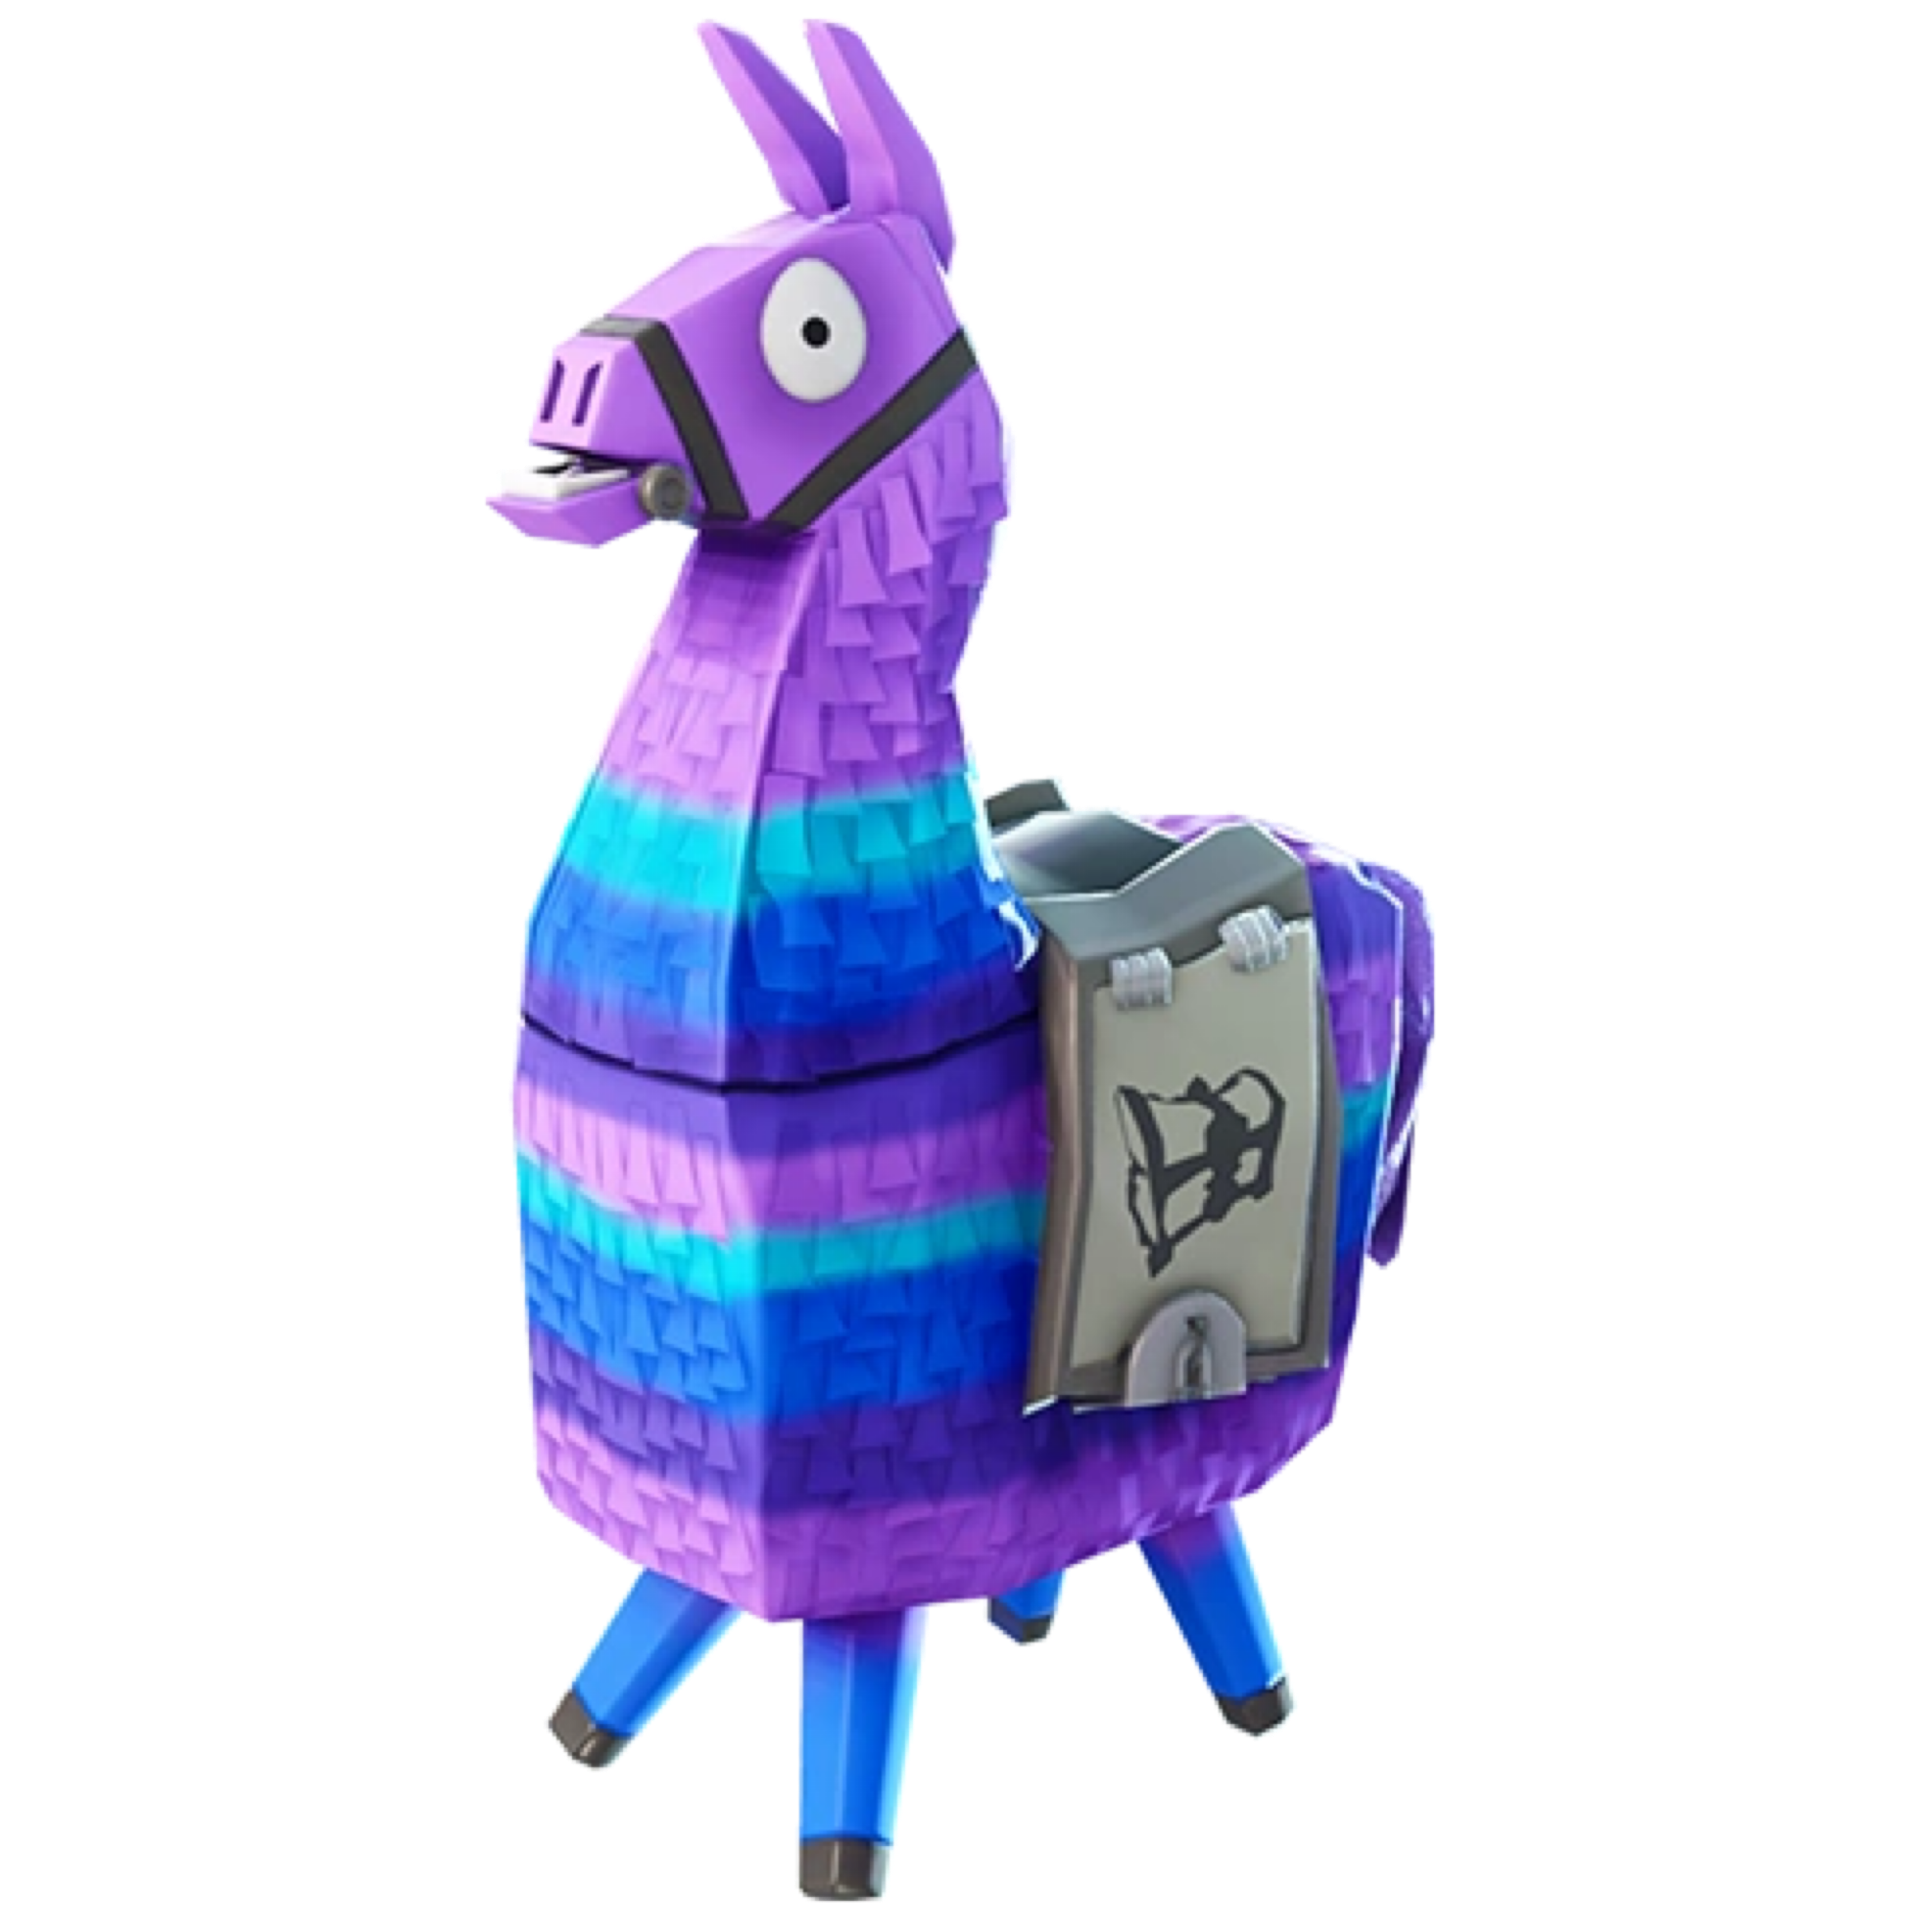
\includegraphics[width=0.2\textwidth]{ressources/iconexample2.png} \hfill
    
\includegraphics[width=0.2\textwidth]{ressources/iconexample3.png} \hfill
    
\includegraphics[width=0.2\textwidth]{ressources/iconexample4.png} \hfill
    \caption{Example of gaming elements used in dataset creation}
    \label{fig:icons}
\end{figure}

\begin{figure}[H]
    \centering
    
\includegraphics[width=0.2\textwidth]{ressources/bad_icon1.png} \hfill
    
\includegraphics[width=0.2\textwidth]{ressources/bad_icon2.png} \hfill
    
\includegraphics[width=0.2\textwidth]{ressources/bad_icon3.png} \hfill
    
\includegraphics[width=0.2\textwidth]{ressources/bad_icon4.png} \hfill
    \caption{Example of gaming elements avoided in dataset creation}
    \label{fig:bad_icons}
\end{figure}
\subsubsection{Footage Collection}
To complete a realistic gaming footage scenario, we have picked random footage
from various TwitchTV streams, focusing on gameplay that prominently features
the UI elements and random backgrounds that could be encountered in real-world
gaming sessions. The footage is then processed to extract frames at a certain
rate, ensuring that the dataset captures dynamic interactions with the UI
elements. Each frame is annotated with the corresponding icons and UI elements
present, allowing for precise evaluation of feature matching performance.

\begin{figure}[H]
    \centering
    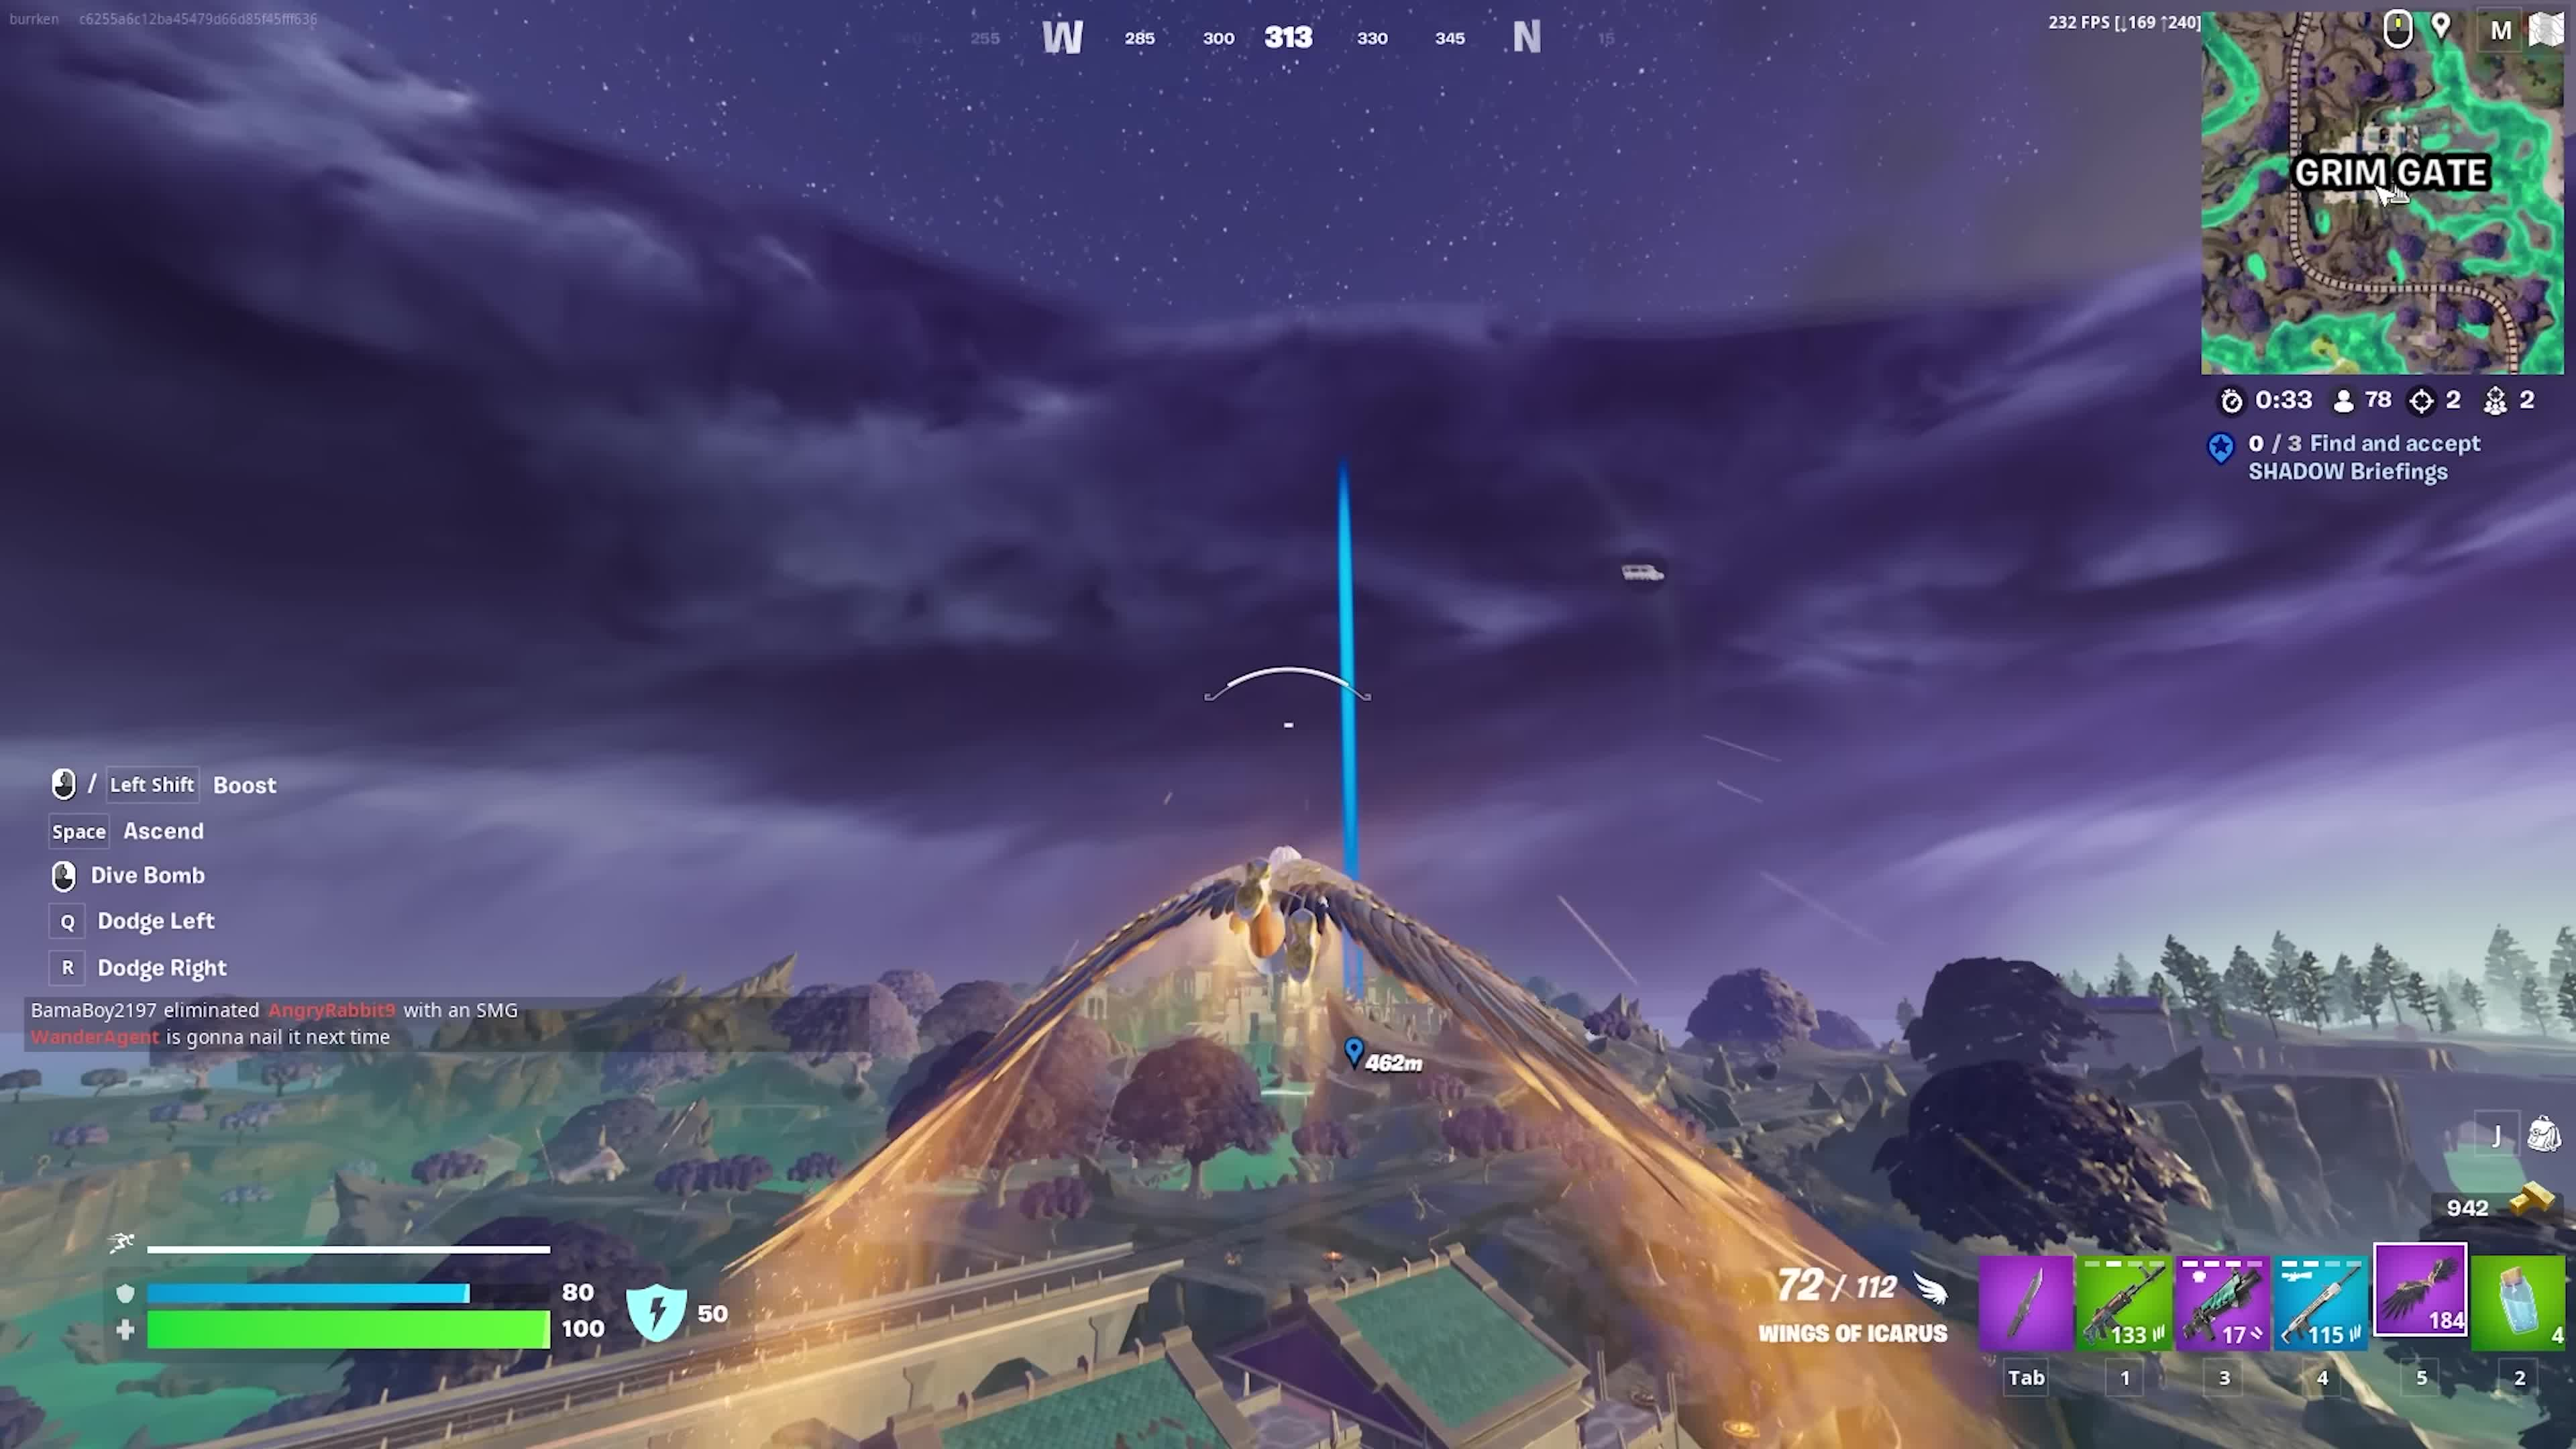
\includegraphics[width=0.8\textwidth]{ressources/bg_example.jpg}
    \caption{Example of backgrounds used in dataset creation}
    \label{fig:background_example}
\end{figure}

This will ensure that the dataset is representative of the actual gaming
environments and provides a solid foundation for training and evaluating the
feature matching.
\subsection{Design of Teacher-Student Framework}
The teacher-student framework is designed to leverage the strengths of both
handcrafted feature matching methods and neural network-based approaches. For
this, we have selected two strong candidates: ALIKE, originally picked by the
authors, and a sophisticated SIFT variant, currently in use at SteelSeries.
Both methods have been used to extract keypoints and match them across our data
samples.
\subsection{SIFT Implementation}
The current solution implemented at SteelSeries leverages a sophisticated SIFT
implementation that enhances the traditional SIFT algorithm for our specific
use case. The implementation goes as follows:

We employ a carefully tuned Scale-Invariant Feature Transform (SIFT) configuration to maximise the number of stable, repeatable keypoints in varied imaging conditions. The detector is initialised with the following parameters:

\begin{itemize}
    \item \textbf{$nOctaveLayers = 4$}: controls the number of scale-space intervals per octave. Increasing this value produces more keypoints across finer scale increments, improving detection in textured or low-detail regions at the cost of additional computation.
    \item \textbf{$contrastThreshold = 0.02$}: sets the minimum contrast required for a candidate keypoint to be retained. Lowering this threshold allows the detector to preserve low-contrast features that may still be distinctive, particularly in low-texture or dim areas, but also increases sensitivity to noise.
    \item \textbf{$edgeThreshold = 5$}: filters out keypoints lying on edges by evaluating the ratio of principal curvatures in the Difference-of-Gaussians response. Lower values are stricter, rejecting more elongated edge responses; our choice balances the removal of unstable edge points with the retention of useful linear features.
    \item \textbf{$\sigma = 1.8$}: specifies the Gaussian smoothing applied at the initial scale of each octave. Larger values increase robustness to noise and small perturbations but can blur fine details; $\sigma = 1.8$ offers a compromise between stability and spatial precision.
\end{itemize}

After detecting keypoints in both the reference and target images, descriptors are computed and normalised by dividing each vector by the sum of its elements. This amplitude normalisation mitigates the effect of overall descriptor magnitude differences, focusing the comparison on relative component values.

Candidate correspondences are generated using a FLANN-based approximate nearest-neighbour search with a KDTree index. For each reference descriptor, the two nearest neighbours in the target descriptor set are retrieved. Match filtering follows a two-pronged strategy:
\begin{enumerate}
    \item \textbf{Relative criterion}: Lowe’s ratio test is applied, retaining matches where the closest neighbour’s distance is less than $0.7$ times that of the second-closest neighbour. This rejects ambiguous matches where multiple candidates are similarly close in descriptor space.
    \item \textbf{Absolute criterion}: Any match with a nearest neighbour distance below $0.09$ is also accepted, even if the ratio test is not satisfied, ensuring that exceptionally strong correspondences are preserved.
\end{enumerate}

The filtered matches are recorded as index pairs into the respective keypoint arrays. This combination of tuned detector parameters, descriptor normalisation, and dual match filtering yields a set of correspondences that is both distinctive and resilient to background clutter and illumination changes.
 \section{Evaluation metrics} %TODO